% !TEX program = xelatex
% ============================================================
%  全国大学生数学建模竞赛 (CUMCM) LaTeX 通用论文模板
%  编译方式: XeLaTeX
% ============================================================
\documentclass[12pt,a4paper,AutoFakeBold=2]{ctexart}

% ======================== 宏包加载 ========================
\usepackage[top=2.5cm, bottom=2.5cm, left=2.8cm, right=2.8cm]{geometry}
\usepackage{amsmath, amssymb, amsthm}
\usepackage{graphicx}
\usepackage{float}
\usepackage{subcaption}
\usepackage{booktabs}
\usepackage{array}
\usepackage{multirow}
\usepackage{longtable}
\usepackage{xcolor}
\usepackage[super]{cite}
\usepackage{hyperref}
\hypersetup{
    colorlinks=true,
    linkcolor=blue!70!black,
    citecolor=green!50!black,
    urlcolor=blue!60!black
}
\usepackage{listings}
\lstset{
    basicstyle=\small\ttfamily,
    breaklines=true,
    frame=single,
    numbers=left,
    numberstyle=\tiny\color{gray},
    keywordstyle=\color{blue},
    commentstyle=\color{green!60!black},
    stringstyle=\color{red!70!black},
    tabsize=4
}

\usepackage{setspace}
\onehalfspacing
\usepackage{enumitem}
\setlist{nosep, leftmargin=2em}
\usepackage{titlesec}
\usepackage{caption}
\captionsetup{font=bf, justification=centering}
\usepackage{bm}
\usepackage{mathtools}

% ======================== 字体设置 ========================
\setCJKmainfont{SimSun}[BoldFont=SimHei, ItalicFont=KaiTi]
\setCJKsansfont{SimHei}[BoldFont=SimHei]
\setCJKmonofont{FangSong}[BoldFont=SimHei]
\setmainfont{Times New Roman}

% ======================== 段落格式 ========================
\usepackage{indentfirst}
\setlength{\parindent}{2em}
\setlength{\parskip}{0pt}

% ======================== 图片路径 ========================
\graphicspath{{figures/}}

% ======================== 编号格式 ========================
\renewcommand{\thesection}{\chinese{section}、}
\renewcommand{\thesubsection}{\arabic{section}.\arabic{subsection}}
\renewcommand{\thesubsubsection}{\arabic{section}.\arabic{subsection}.\arabic{subsubsection}}

% ======================== 标题格式 ========================
\titleformat{\section}
  {\centering\heiti\zihao{-3}}
  {\thesection}{0em}{}
\titlespacing*{\section}{0pt}{1.5ex plus .5ex minus .2ex}{1.0ex plus .2ex}

\titleformat{\subsection}
  {\heiti\zihao{4}}
  {\thesubsection}{1em}{}
\titlespacing*{\subsection}{0pt}{1.2ex plus .4ex minus .2ex}{0.8ex plus .2ex}

\titleformat{\subsubsection}
  {\heiti\zihao{-4}}
  {\thesubsubsection}{1em}{}
\titlespacing*{\subsubsection}{0pt}{1.0ex plus .3ex minus .1ex}{0.6ex plus .1ex}

% ======================== 自定义命令 ========================
\newenvironment{symboltable}
  {\begin{center}\zihao{5}\begin{tabular}{>{\centering\arraybackslash}p{3.5cm} >{\centering\arraybackslash}p{7.5cm} >{\centering\arraybackslash}p{1.5cm}}
  \toprule
  \textbf{符号} & \textbf{含义} & \textbf{单位} \\
  \midrule}
  {\bottomrule\end{tabular}\end{center}}

\newcommand{\step}[1]{\par\noindent\textbf{Step #1}\quad}

% ============================================================
\begin{document}
\pagestyle{plain}

\begin{center}
{\zihao{-2}\heiti 基于多维交易流水特征的小微企业信用评级重构与预测}
\end{center}
\vspace{1em}

% ======================== 摘要 ========================
\setcounter{page}{1}
\pagenumbering{arabic}

\begin{center}\heiti\zihao{-3}摘\quad 要\end{center}\zihao{-4}\songti

小微企业信用评级直接影响银行信贷决策，但银行评级依赖主观判断，其准确性有待检验。本文基于交易票据流水数据，建立主成分分析与多元逻辑回归模型验证银行评级的准确性，并构建熵权赋权与加权聚类模型重构客观分类标准，对302家无信贷记录企业进行信用评级预测。

\textbf{针对问题一：}本文构建了基于主成分分析与多元逻辑回归的分类验证模型以评估银行评级准确性。研究从进销项发票中提取19个基础变量并创新构造供应链稳定度与平均营收增长率，通过降维提取出活力因子金额因子故障因子与作废因子四个公因子。模型求解结果显示总体准确率为54.47\%且一致性系数仅为0.384，其中A级与D级识别率分别达到62.96\%和66.67\%，但B级与C级准确率仅为57.89\%和35.29\%且存在21家企业的严重互混。该结果表明银行原始评级在极端信用水平判断上基本准确，但在中间等级存在显著错配，整体分类结果不够准确。

\textbf{针对问题二：}本文建立了基于信息客观赋权与高维空间加权聚类重构标签的有监督预测模型。计算得出金额因子与活力因子的客观权重合计高达68.1\%，在八维空间中聚类生成的新标签分布均衡且与银行原标签的调整兰德指数仅为0.039。以重构标签为目标训练的多元逻辑回归分类模型五折交叉验证准确率达到91.1\%，最终对302家企业的预测结果显示中间偏下等级占比最大且预测置信度均值高达0.882。该结果成功建立了一套独立于主观判断的客观分类标准，并高置信度地完成了对新企业的信用评级预测。

\par\noindent\textbf{关键词：}信用评级\quad 主成分分析\quad 多元Logit\quad 熵权法\quad 加权K-Means

\newpage

% ============================================================
%  正文
% ============================================================

\section{问题重述}

\subsection{问题背景}

小微企业在国民经济中发挥着重要作用，但受制于资产规模较小且缺乏足额抵押物，金融机构在提供信贷支持时面临较高的信息不对称风险\cite{ref2}。为了有效管控信贷风险，银行通常需要对借款企业进行严格的信用等级划分。在实际业务场景中，企业的进销项发票等交易票据信息能够客观映射其真实的经营活跃度、资金流转规模以及潜在的交易违约风险，因而成为银行内部人员进行信用评定的核心数据支撑。然而，完全依赖人工经验或主观判断的评级过程不可避免地会引入认知偏差，导致最终的分类结果可能无法精准反映企业的真实信用资质。因此，如何充分挖掘海量票据数据背后的深层经营特征，利用量化模型对现有评级体系的科学性进行检验，并为缺乏信贷历史的新客户建立客观的分类标准，成为当前小微企业信贷风控领域亟待解决的关键问题。
\subsection{问题提出}

附件1与附件2分别提供了123家有信贷记录企业及302家无信贷记录企业的进销项发票流水数据，涵盖了交易频次、资金规模及票据状态等关键经营信息。为帮助银行优化小微企业信贷风险控制体系并提升评级科学性，现需结合实际情况与附件所给信息建立数学模型，分析以下问题：

\textbf{问题一：}需要依托有信贷记录企业的多维票据信息构建数学模型，分析交易规模、活跃度及供应链特征与既有信用评级之间的对应关系，从而确定123 家企业的信用等级的分类结果是否准确。

\textbf{问题二：}基于问题一对银行评级准确性的验证结论，需对附件2中302家无信贷记录企业进行信用评级。若原评级体系被证实准确，则沿用现有标准进行分类；若原评级存在显著偏差，则需摒弃主观标签，依据交易票据数据构建客观分类准则，并将该准则迁移应用于无信贷记录企业群体，最终为金融机构信贷审批提供高置信度的量化决策依据。

\section{问题分析}


\subsection{问题一的分析}

问题一的核心难点在于如何将银行主观评级转化为可量化的客观验证过程。这要求我们不仅要构建能够准确反映企业真实经营状况的评价维度，还要建立具有统计显著性的分类模型来评估评级质量。特征工程的挑战在于原始发票数据存在多重共线性且量纲差异显著，直接入模会导致系数失真。为此，我们从原始流水中提取19个基础变量，并创新性地构造供应链稳定度与平均营收增长率作为复合指标，既保留了数据的经济学意义又避免了PCA降维对复合指标的干扰。在构建评级验证模型时，本文采用多元Logit回归模型进行多分类拟合，同时引入XGBoost模型开展5折分层交叉验证。最终，我们通过混淆矩阵揭示B/C中间等级的严重错配现象，利用Cohen's Kappa系数排除随机一致的影响，并通过时效性稳健性检验证实银行评级必须依赖长周期数据，从而全面证实了银行原始评级在极端信用水平判断上基本准确，但在中间等级存在显著错配。
\subsection{问题二的分析}

问题二需要在问题一证实银行评级存在偏差的前提下，建立独立于主观判断的客观分类标准并对无信贷记录企业进行预测。整体思路分三个阶段：先用熵权法对核心特征客观赋权，反映各维度对信用区分的信息贡献；再在多维特征空间中执行加权聚类重构标签，避免一维投影带来的信息损失与标签偏斜，生成具有清晰经济含义的新评级体系；最后以重构标签为目标训练有监督分类器，将聚类规则泛化至302家新企业，输出高置信度的预测结果。

\section{模型假设}

\begin{enumerate}[label=\arabic*., leftmargin=2em]
\item 假设企业的交易票据信息能够真实反映其经营状况与信用水平。
\item 假设企业短期交易模式稳定延续，历史票据特征能够代表当前信用资质。
\item 假设银行给出的原始信用等级虽然存在局部错配，但整体分布仍符合宏观经济规律，可作为模型构建的初始参考基准。
\end{enumerate}

\section{符号说明}

\begin{symboltable}
$x_1 \sim x_{19}$ & 企业进销项发票基础汇总变量 & $-$ \\
$F_1 \sim F_4$ & PCA提取的4个公因子 & $-$ \\
$F_7, F_8, F_9$ & 供应链稳定度：进、销、进销综合集中度 & $-$ \\
$F_{10}$ & 平均营收增长率 & $-$ \\
$w_j$ & 第$j$个特征的熵权法客观权重 & $-$ \\
$z_{ij}$ & 标准化后的特征数值 & $-$ \\
$P(y=j \mid \mathbf{x})$ & 多元Logit模型预测企业属于评级$j$的概率 & 百分比 \\
$\kappa$ & Cohen's Kappa一致性系数 & $-$ \\
$C_i$ & 加权K-Means聚类所得企业标签 & 等级 \\
\end{symboltable}


\section{模型建立与求解}

\subsection{数据预处理}

为刻画小微企业的经营特征，本文从原始发票流水中提取19个基础变量，并构造4个衍生特征，最终通过PCA降维形成入模特征体系。

\subsubsection{数据清洗与特征提取}

原始数据中的发票状态仅包含有效与作废两类，不存在独立的负数发票状态标识。本文通过判断有效发票中价税合计小于零的条目识别负数发票，将全部进项与销项发票按状态分类汇总，提取19个基础变量：进项侧8个即发票数量$x_1$、有效数量$x_2$、作废数量$x_3$、负数数量$x_4$、有效金额$x_5$、有效税额$x_6$、无效额$x_7$、有效价税总和$x_8$；销项侧8个对称变量$x_9 \sim x_{16}$；衍生比率3个即有效收入$x_{17}=x_{16}-x_8$、作废发票率$x_{18}$、负数发票率$x_{19}$。

原始数据存在极端值干扰和量纲差异，本文对所有连续变量执行1\%与99\%分位数的Winsorize缩尾处理。为使各变量具有可比性并满足 PCA 对数据标准化的要求，再对参与PCA的19个基础变量进行Z-score标准化：
\begin{equation}
z_i = \frac{x_i - \bar{x}}{s}
\label{eq:zscore}
\end{equation}
其中$\bar{x}$为样本均值，$s$为样本标准差。经标准化处理后，各变量均值为0、标准差为1，消除了量纲差异对 PCA 载荷矩阵计算的干扰，确保各变量在降维过程中具有同等权重。

\subsubsection{创新特征构造}

为弥补传统财务指标无法刻画供应链风险与发展趋势的局限，本文独立构造了以下特征。

为衡量企业供应链依赖风险，定义进稳定度$F_7$、销稳定度$F_8$及综合稳定度$F_9$：
\begin{equation}
F_7 = \frac{\sum_{k \in \text{Top3\_Sup}} N_{in}^k}{x_1}, \quad F_8 = \frac{\sum_{k \in \text{Top3\_Cus}} N_{out}^k}{x_9}, \quad F_9 = \sqrt{\frac{F_7^2 + F_8^2}{2}}
\label{eq:supply_chain}
\end{equation}
其中$N_{in}^k$表示来自供应商$k$的发票数量。集中度过高意味着企业过度依赖少数交易对手，抗风险能力弱。123家企业的$F_9$均值0.494，部分企业$F_7$超过0.7，供应链集中度差异显著。

为捕捉企业动态发展趋势，定义平均营收增长率$F_{10}$：
\begin{equation}
F_{10} = \frac{1}{T-1}\sum_{t=1}^{T-1}\frac{R_{t+1} - R_t}{|R_t| + \epsilon}
\label{eq:growth_rate}
\end{equation}
其中$R_t$为第$t$年的销项有效价税合计，$\epsilon$为防止除零的平滑项。计算后对$F_{10}$截断至$[-1, 5]$剔除极端值，截断后均值1.28，持续增长的企业信用风险较低，持续萎缩的企业则相反。此特征为原论文\cite{ref1}未涉及的创新维度。

稳定度与增长率不参与PCA降维：它们本身为无量纲比值，与19个发票汇总变量在量纲和语义上差别较大，若混入PCA会干扰因子的经济含义解释。因此采用并列策略，PCA仅对发票汇总变量降维，稳定度和增长率作为独立特征与PCA因子并列进入模型。

\subsubsection{降维与特征体系构建}

19个基础变量间存在多重共线性，直接入模会导致系数不稳定，本文采用PCA主成分降维。适用性检验结果：KMO检验值0.722大于0.5，Bartlett球形检验$\chi^2=10440$, $p<0.001$，确认变量间存在足够相关性，适合做因子分析。

按Kaiser准则即特征根大于1提取4个公因子，经Varimax旋转后命名及方差贡献如表\ref{tab:pca}所示。

\begin{table}[H]
\centering
\caption{PCA提取4个公因子及方差贡献}
\label{tab:pca}
\zihao{5}
\begin{tabular}{cccc}
\toprule
公因子 & 方差贡献 & 累计贡献 & 命名 \\
\midrule
$F_1$ & 31.71\% & 31.71\% & 活力因子 \\
$F_2$ & 34.25\% & 65.96\% & 金额因子 \\
$F_3$ & 14.08\% & 80.04\% & 故障因子 \\
$F_4$ & 6.18\% & 86.22\% & 作废因子 \\
\bottomrule
\end{tabular}
\end{table}

4个公因子累计解释86.22\%的总方差，信息保留充分。特征值在第4个因子后急剧下降趋于平缓，印证了取4个因子的合理性。

载荷矩阵揭示了各因子的经济含义：$F_1$高载荷变量为发票数量类$x_1$ 0.955与$x_2$ 0.954，反映交易活跃度；$F_2$高载荷变量为金额类$x_7$ 0.969与$x_{16}$ 0.937，反映资金规模；$F_3$高载荷变量为负数发票率$x_{19}$ 0.766，反映退货风险；$F_4$高载荷变量为作废发票率$x_{18}$ $-0.649$，反映交易取消频率。如图\ref{fig:loading}所示，旋转后载荷矩阵热力图清晰展示了各变量在因子上的归属关系。

\begin{figure}[H]
\centering
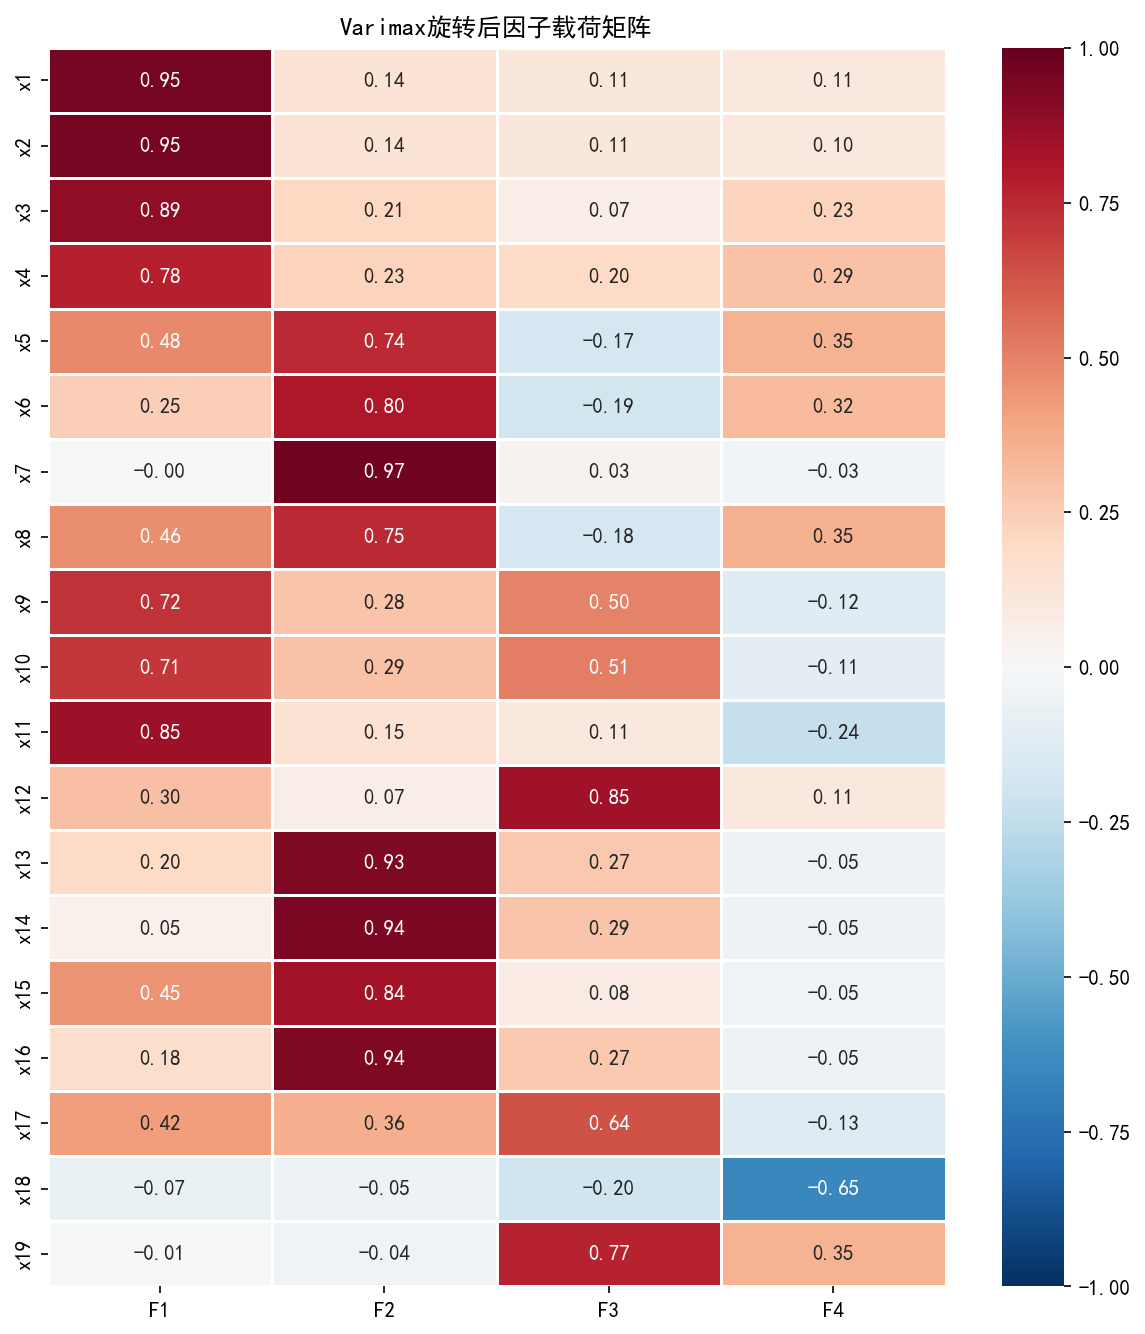
\includegraphics[width=0.8\textwidth]{fig2_loading_heatmap.png}
\caption{旋转后因子载荷热力图}
\label{fig:loading}
\end{figure}

最终入模特征向量为$\mathbf{x} = [F_1, F_2, F_3, F_4, F_7, F_8, F_9, F_{10}]^T$，共8维，兼顾了交易规模、活跃度、风险状况与发展趋势。

\subsection{问题一模型建立及求解}

\subsubsection{模型建立}

为验证银行信用评级准确性，本文构建多元Logit分类模型。以A级为基准组，对其余类别$j \in \{B, C, D\}$建立对数机会比模型：
\begin{equation}
G_j = \ln\frac{P(y=j \mid \mathbf{x})}{P(y=A \mid \mathbf{x})} = \beta_{j0} + \sum_{k=1}^{8}\beta_{jk}x_k
\label{eq:logit}
\end{equation}
其中$\mathbf{x}$为包含4个PCA因子和4个衍生特征的8维向量，$\beta_{j0}$为截距项，$\beta_{jk}$为第$k$个特征对第$j$类别的回归系数。$\beta_{jk}>0$表示特征$x_k$将企业推向更差等级，$\beta_{jk}<0$则相反。预测概率由softmax函数给出：
\begin{equation}
P(y=j \mid \mathbf{x}) = \frac{e^{G_j}}{\sum_{m \in \{A,B,C,D\}}e^{G_m}}
\label{eq:softmax}
\end{equation}
分类规则取预测概率最大的类别：$\hat{y} = \arg\max_{j} P(y=j \mid \mathbf{x})$。

同时引入XGBoost作为辅助验证模型\cite{ref3}，采用5折分层交叉验证：其一，准确率可作为特征体系分类上限的参照；其二，特征重要性排序可佐证各因子的相对贡献。

\subsubsection{模型求解}

\step{1} 将123家有信贷记录企业的8维特征向量$\mathbf{x}$与银行标签$y$组成训练集，对多元Logit模型进行最大似然估计。

\step{2} 对XGBoost模型进行5折分层交叉验证，获取分类上限参照与特征重要性排序。

\step{3} 计算Logit总体准确率、Cohen's Kappa一致性系数及各级别召回率，输出混淆矩阵。

\step{4} 仅使用2019--2020年近期数据重新预测，进行时效性稳健性检验。

\subsubsection{结果展示}

Logit模型整体高度显著，LLR $p < 0.001$，伪$R^2$为0.238。回归系数分析显示，活力因子$F_1$和金额因子$F_2$在D vs A对比中显著为负，$\beta=-7.55$和$-20.15$，说明交易越活跃、规模越大的企业越不可能被评为D级；进销稳定度$F_9$系数显著为正，$\beta=30.62$，说明供应链集中度越高，被评为差等级的对数机会比增大。

Logit总体准确率54.47\%即67/123，Cohen's Kappa为0.384。Kappa系数的计算公式为：
\begin{equation}
\kappa = \frac{p_o - p_e}{1 - p_e}
\label{eq:kappa}
\end{equation}
其中$p_o$为观测一致率即总体准确率，$p_e$为期望随机一致率。$\kappa<0.4$判定为一致性一般，$0.4\sim0.6$为中等，$0.6\sim0.8$为较好。

分级别准确率如表\ref{tab:logit_perf}所示。

\begin{table}[H]
\centering
\caption{问题一模型分类性能对比}
\label{tab:logit_perf}
\zihao{5}
\begin{tabular}{cccc}
\toprule
模型 & 总体准确率 & Cohen's Kappa & 结论 \\
\midrule
多元Logit & 54.47\% & 0.384 & 一致性一般，B/C级错配严重 \\
XGBoost 5折CV & 43.09\% & 0.231 & 特征区分度上限受限 \\
\bottomrule
\end{tabular}
\end{table}

如图\ref{fig:logit_cm}所示，Logit模型对A级识别率62.96\%和D级识别率66.67\%较高，但C级准确率仅为35.29\%，13家C级被误判为B级，B/C互混严重。

\begin{figure}[H]
\centering
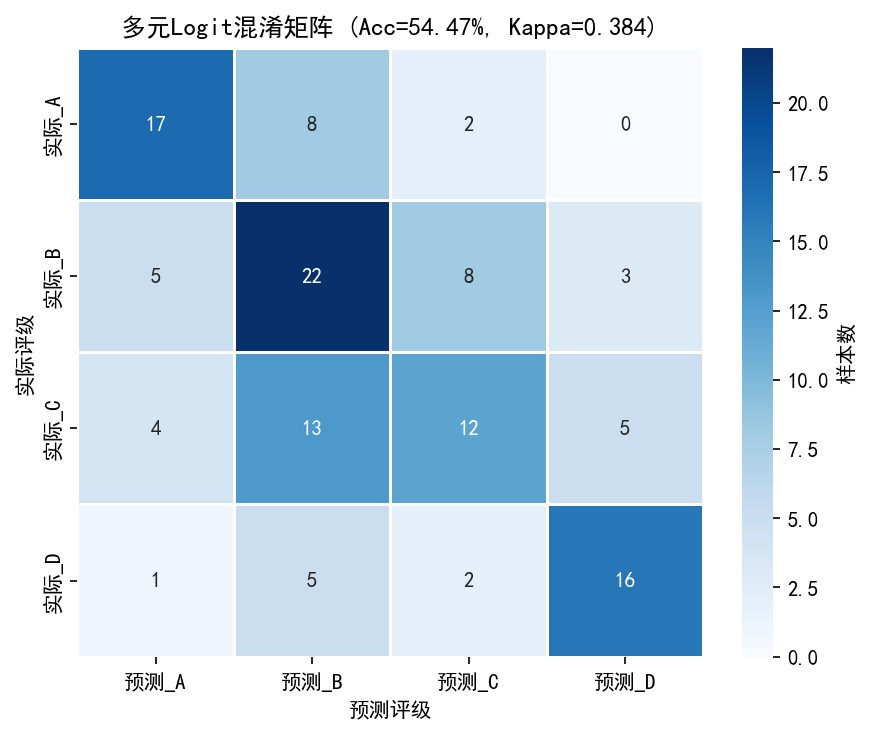
\includegraphics[width=0.6\textwidth]{fig4_logit_confusion.png}
\caption{多元Logit模型预测混淆矩阵}
\label{fig:logit_cm}
\end{figure}

如图\ref{fig:xgb_cm}所示，XGBoost 5折CV准确率仅43.09\%，低于Logit的54.47\%。这并非说明Logit更好，而是反映小样本下非线性模型容易过拟合，其准确率可视为特征体系分类上限的保守估计。

\begin{figure}[H]
\centering
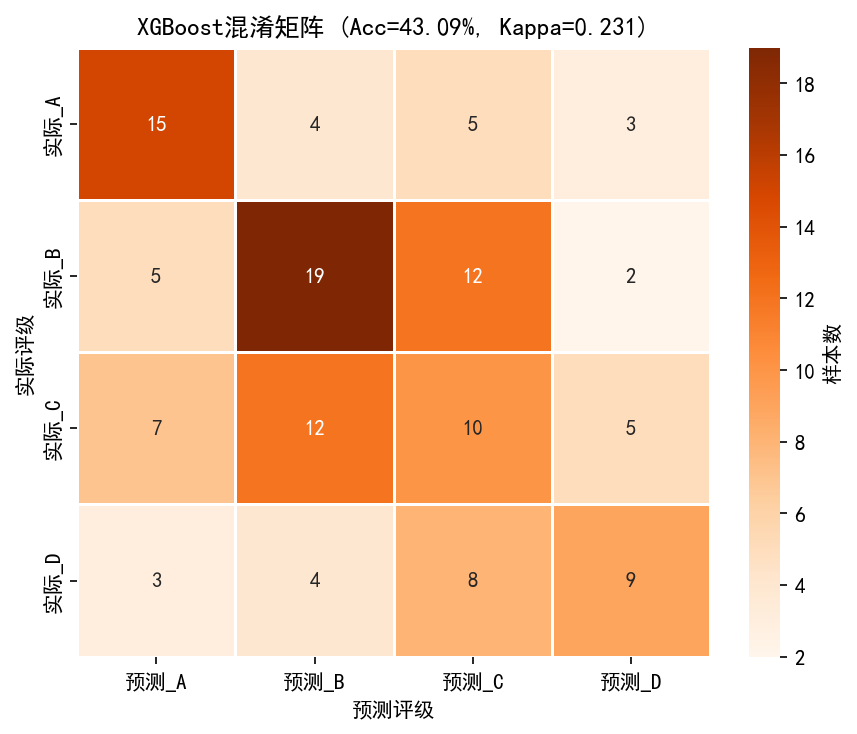
\includegraphics[width=0.6\textwidth]{fig5_xgb_confusion.png}
\caption{XGBoost 5折交叉验证混淆矩阵}
\label{fig:xgb_cm}
\end{figure}

特征重要性排序如图\ref{fig:xgb_imp}所示，$F_9$进销稳定度和$F_3$故障因子排名前二，验证了供应链集中度和退货退款风险对信用评估的补充价值；$F_{10}$增长率排名第三，作为创新特征贡献显著。

\begin{figure}[H]
\centering
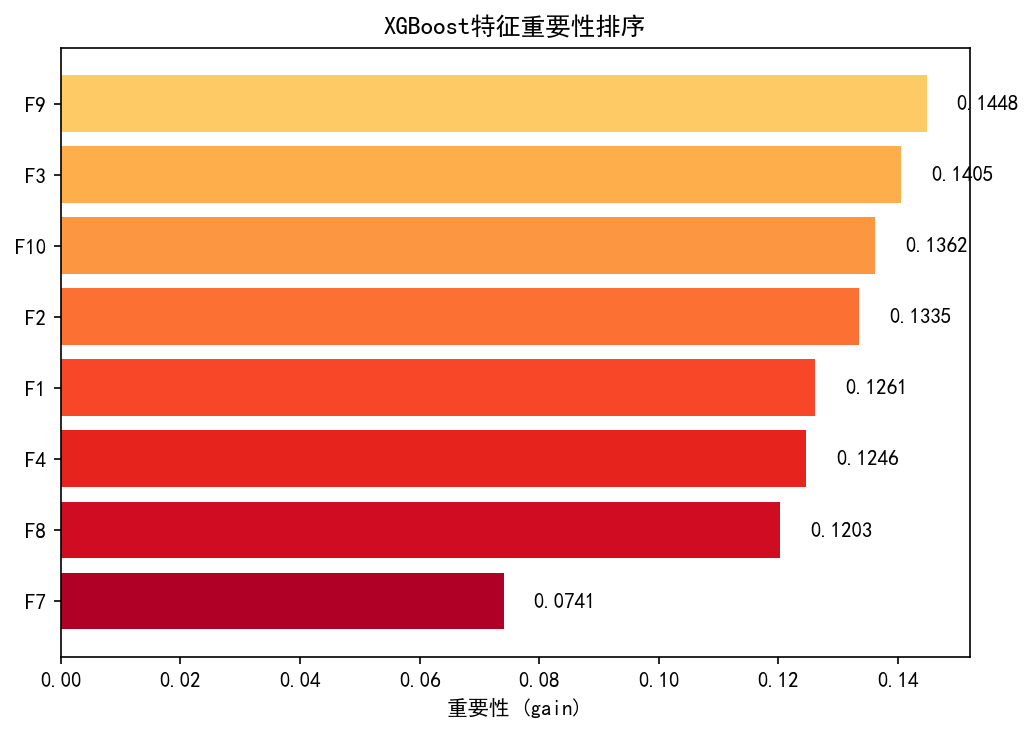
\includegraphics[width=0.7\textwidth]{fig6_xgb_importance.png}
\caption{XGBoost特征重要性排序}
\label{fig:xgb_imp}
\end{figure}

\subsubsection{结果分析与验证}

\textbf{评级准确性剖析：}Kappa系数仅为0.384，表明模型预测与银行标签的一致性一般。银行对A、D两端极端信用水平的判断基本准确，但B/C中间等级存在显著错配——C级仅35.29\%被正确识别，13家被误判为B级，说明银行在中间等级的划分标准模糊，存在主观噪声。

\textbf{XGBoost辅助验证：}非线性模型同样无法大幅提升准确率，仅43.09\%，说明特征本身区分力不足是根本原因，而非模型选择问题。

\textbf{时效性稳健性检验：}仅使用2019--2020年近期数据重新预测，结果如图\ref{fig:robust}所示，准确率骤降至30.89\%、Kappa 0.133，相比全数据54.47\%下降23.6个百分点。原因在于短期截断数据无法计算跨年增长率$F_{10}$，特征信息量坍塌，证实了信用评估必须依赖长周期的交易数据。

\begin{figure}[H]
\centering
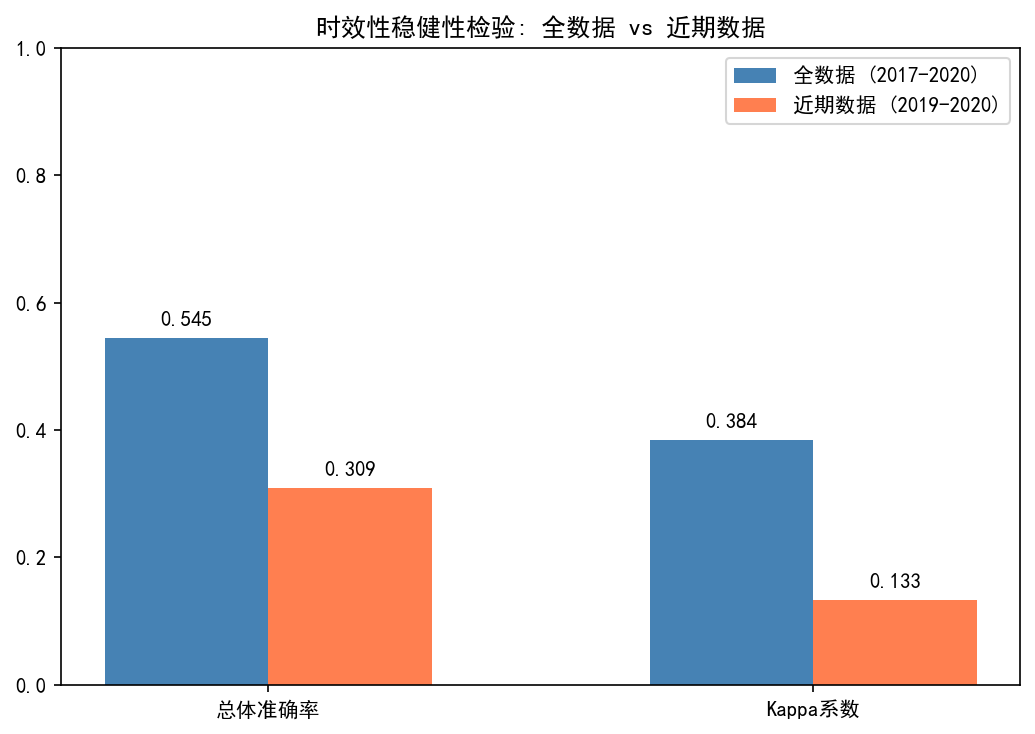
\includegraphics[width=0.7\textwidth]{fig7_robustness.png}
\caption{时效性稳健性检验}
\label{fig:robust}
\end{figure}

\subsection{问题二模型建立及求解}

鉴于问题一证实原标签存在噪声，本文采用熵权法赋权→加权K-Means重构→有监督预测的递进策略。

\subsubsection{模型建立}

\textbf{阶段一：熵权法客观赋权。}为确定各特征对信用区分的客观贡献，本文采用熵权法对8个特征赋权。首先按特征方向做min-max标准化，统一为正向$[0,1]$：正向特征$z_{ij}=(x_{ij}-\min)/(\max-\min)$，负向特征$z_{ij}=(\max-x_{ij})/(\max-\min)$。

然后计算信息熵与权重：
\begin{equation}
e_j = -\frac{1}{\ln n}\sum_{i=1}^{n}p_{ij}\ln p_{ij}, \quad d_j = 1 - e_j, \quad w_j = \frac{d_j}{\sum_{k=1}^{m}d_k}
\label{eq:entropy}
\end{equation}
其中$p_{ij}=z_{ij}/\sum_i z_{ij}$为第$i$个企业在第$j$个特征上的比重。

\textbf{阶段二：加权K-Means重构标签。}为避免一维投影信息损失和标签极端偏斜，本文直接在8维加权特征空间中执行K-Means聚类。加权欧氏距离定义为：
\begin{equation}
d(\mathbf{x}_i, \mathbf{c}_l) = \sqrt{\sum_{j=1}^{m}w_j(x_{ij} - c_{lj})^2}
\label{eq:wkmeans}
\end{equation}
实现时做等价变换$z'_{ij}=\sqrt{w_j}\cdot z_{ij}$，对$\mathbf{Z}'$执行标准K-Means即可。按簇中心加权综合得分降序映射为A'/B'/C'/D'四个等级。

\textbf{阶段三：有监督分类预测。}以重构标签$Y'$为目标，训练分类器将聚类规则泛化至302家无信贷记录企业，输出高置信度的预测结果。

\subsubsection{模型求解}

\step{1} 对8个特征按方向做min-max标准化后计算信息熵$e_j$、差异系数$d_j$与客观权重$w_j$。

\step{2} 对标准化特征做加权变换$z'_{ij}=\sqrt{w_j}\cdot z_{ij}$，在$\mathbf{Z}'$空间执行K-Means聚类，$k=4$，按簇中心得分降序映射为A'/B'/C'/D'。

\step{3} 以重构标签$Y'$为目标，训练Logit与XGBoost分类器，分别使用8维PCA和23维原始两组特征，5折交叉验证选取最优组合。

\step{4} 用最优分类器对302家无信贷记录企业进行评级预测，输出置信度分布与各等级画像。

\subsubsection{结果展示}

熵权法赋权结果如表\ref{tab:entropy}所示。金额因子$F_2$权重0.374、活力因子$F_1$权重0.307，合计68.1\%，说明企业间差异最大的是交易规模和活跃度。故障因子$F_3$和作废因子$F_4$权重合计仅2.2\%，增长率$F_{10}$权重13.7\%排第三。如图\ref{fig:entropy_w}所示，权重分布高度集中于前两个因子。

\begin{table}[H]
\centering
\caption{熵权法客观赋权结果}
\label{tab:entropy}
\zihao{5}
\begin{tabular}{cccc}
\toprule
特征 & 信息熵$e_j$ & 差异系数$d_j$ & 权重$w_j$ \\
\midrule
$F_2$金额 & 0.783 & 0.217 & \textbf{0.374} \\
$F_1$活力 & 0.822 & 0.178 & \textbf{0.307} \\
$F_{10}$增长率 & 0.920 & 0.080 & 0.137 \\
$F_8$销稳定度 & 0.957 & 0.043 & 0.074 \\
$F_7$进稳定度 & 0.971 & 0.029 & 0.050 \\
$F_9$进销稳定度 & 0.979 & 0.022 & 0.037 \\
$F_4$作废 & 0.991 & 0.009 & 0.015 \\
$F_3$故障 & 0.996 & 0.004 & 0.008 \\
\bottomrule
\end{tabular}
\end{table}

\begin{figure}[H]
\centering
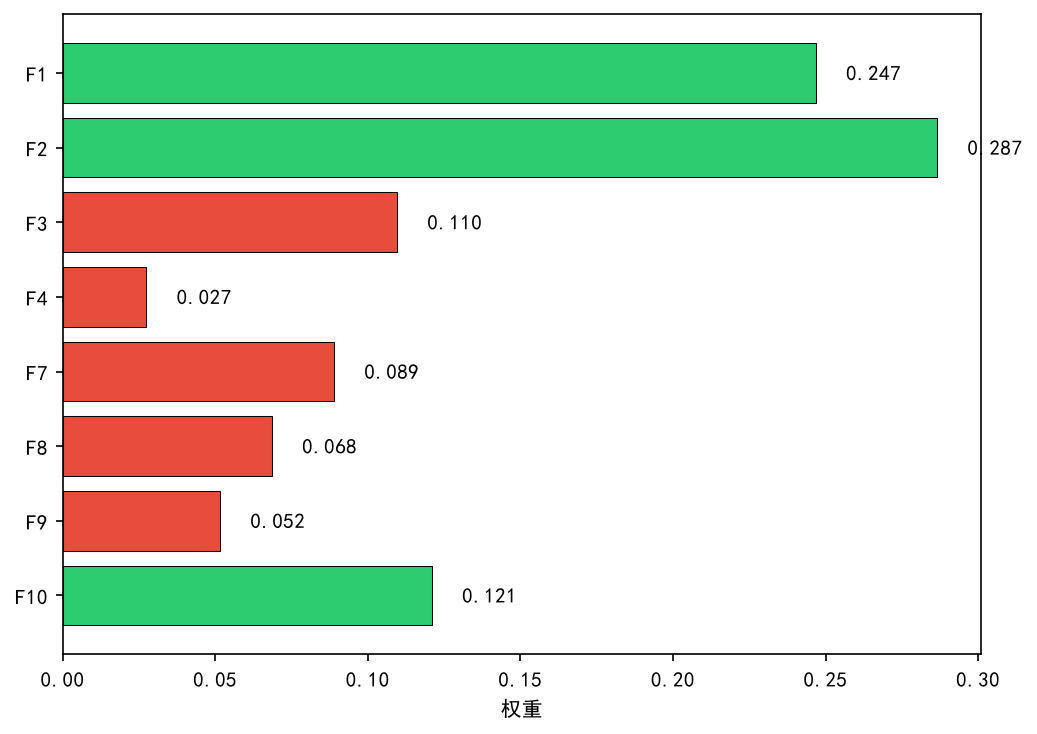
\includegraphics[width=0.7\textwidth]{fig8b_entropy_weights.png}
\caption{熵权法各特征权重分布}
\label{fig:entropy_w}
\end{figure}

聚类数目选择方面，本文计算k=2--6的轮廓系数如图\ref{fig:silhouette}所示。k=3轮廓系数最高为0.465，k=4为0.303。k=4并非统计最优，但信用评级体系要求四档分类为业务约束，k=4轮廓系数0.303为正值，聚类结构有意义。

\begin{figure}[H]
\centering
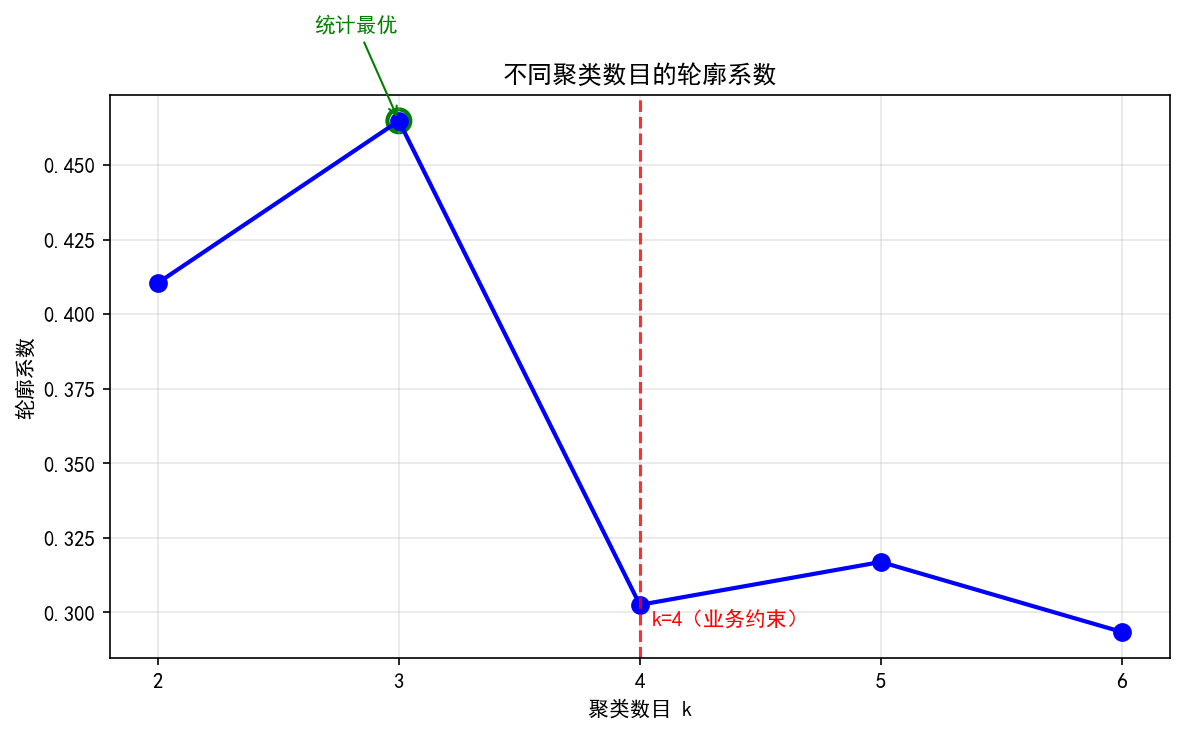
\includegraphics[width=0.65\textwidth]{fig13_silhouette_by_k.png}
\caption{不同聚类数目的轮廓系数}
\label{fig:silhouette}
\end{figure}

新标签分布为A'/B'/C'/D'=9/25/50/39，相比前一版TOPSIS方案标签分布明显更均衡。各等级特征画像如图\ref{fig:cluster_profile}所示：A'为极高活力与金额的头部优质企业；B'为增长率极高但规模偏低的高速成长型企业，$F_{10}=4.69$；C'为各因子接近均值的普通中型企业；D'为低活跃、高依赖度的低信用企业，$F_8=0.69$。

\begin{figure}[H]
\centering
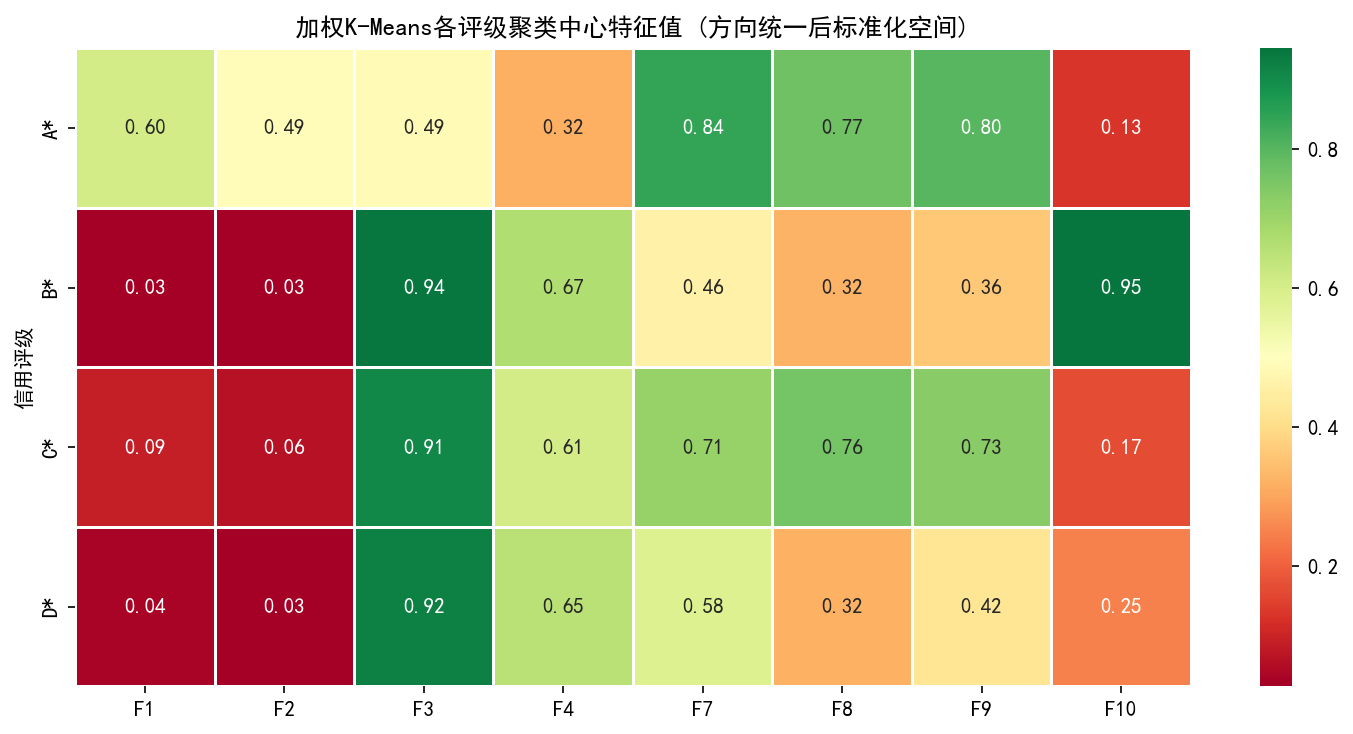
\includegraphics[width=0.75\textwidth]{fig8_cluster_profile.png}
\caption{加权K-Means各等级聚类中心特征画像}
\label{fig:cluster_profile}
\end{figure}

如图\ref{fig:label_cmp}所示，新标签与银行标签的调整兰德指数ARI仅0.039，一致性极低，揭示了客观数据驱动标准与银行主观判断之间的结构性分歧。

\begin{figure}[H]
\centering
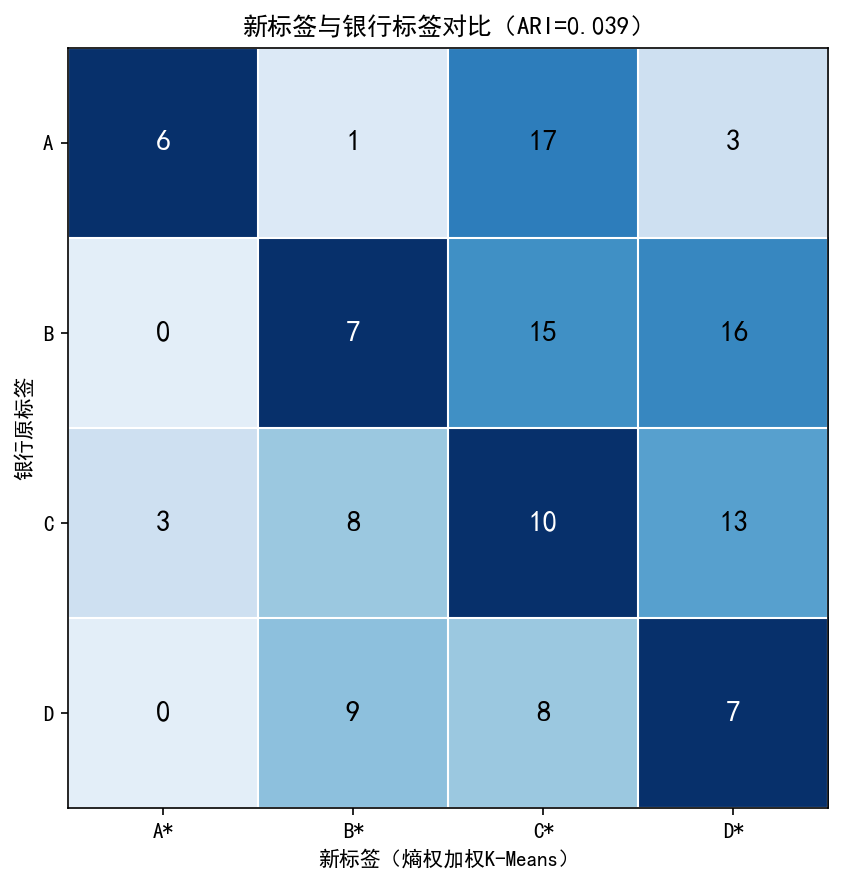
\includegraphics[width=0.65\textwidth]{fig14_label_comparison.png}
\caption{新标签与银行标签对比}
\label{fig:label_cmp}
\end{figure}

有监督分类器5折交叉验证对比如表\ref{tab:classifier}所示，Logit-B使用23维原始特征以91.1\%准确率、Kappa 0.871表现最优。

\begin{table}[H]
\centering
\caption{有监督分类器5折交叉验证对比}
\label{tab:classifier}
\zihao{5}
\begin{tabular}{cccc}
\toprule
模型 & 特征维度 & 准确率 & Kappa \\
\midrule
\textbf{Logit-B} & \textbf{23维原始} & \textbf{91.1\%} & \textbf{0.871} \\
XGBoost-A & 8维PCA & 91.1\% & 0.869 \\
Logit-A & 8维PCA & 90.2\% & 0.859 \\
XGBoost-B & 23维原始 & 89.4\% & 0.844 \\
\bottomrule
\end{tabular}
\end{table}

特征重要性排序如图\ref{fig:p2_imp}所示，一个关键发现是：熵权法中权重极低的稳定度$F_8/F_9$在分类器中重要性排第2、3位，说明稳定度对信用分档存在非线性阈值效应。

\begin{figure}[H]
\centering
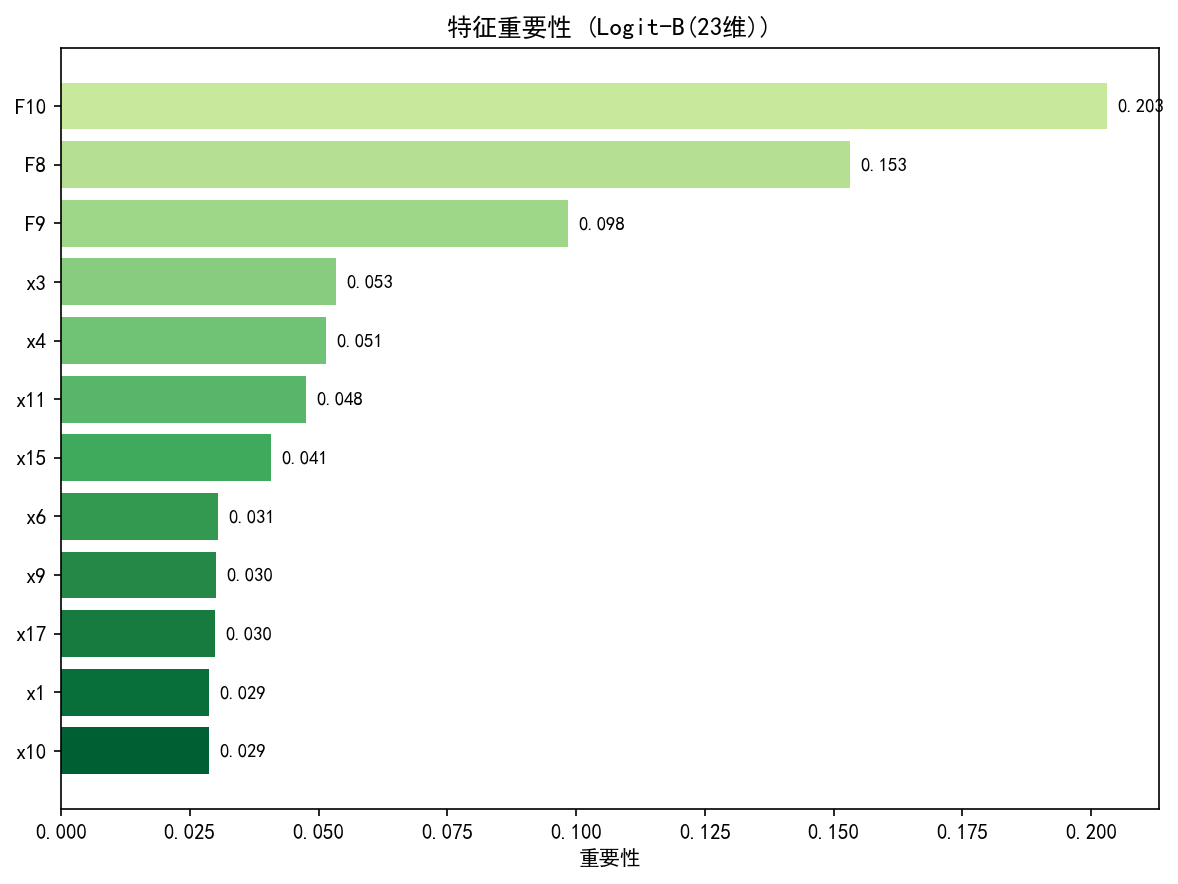
\includegraphics[width=0.7\textwidth]{fig9_p2_importance.png}
\caption{分类器特征重要性排序}
\label{fig:p2_imp}
\end{figure}

302家企业预测结果如图\ref{fig:p2_dist}所示：A'7家即2.3\%、B'61家即20.2\%、C'134家即44.4\%、D'100家即33.1\%，呈中间大两端小分布。

\begin{figure}[H]
\centering
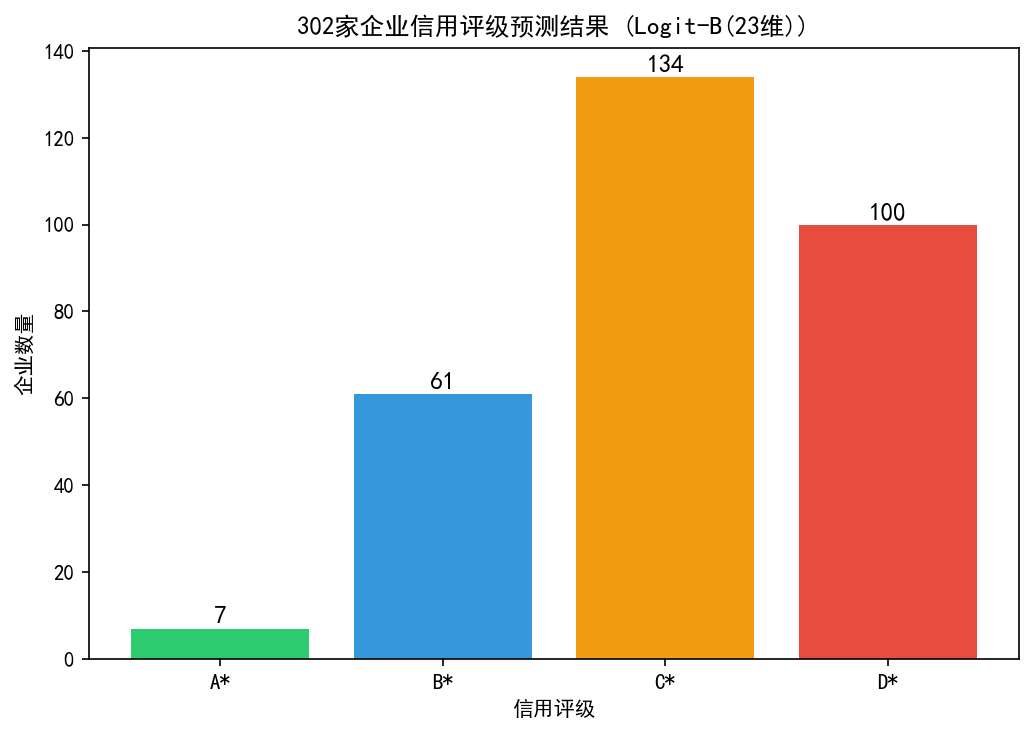
\includegraphics[width=0.7\textwidth]{fig10_p2_prediction.png}
\caption{302家无信贷记录企业预测评级分布}
\label{fig:p2_dist}
\end{figure}

预测置信度分布如图\ref{fig:confidence}所示：均值0.882，中位数0.962，高置信企业即置信度大于0.7共253家，占83.8\%。

\begin{figure}[H]
\centering
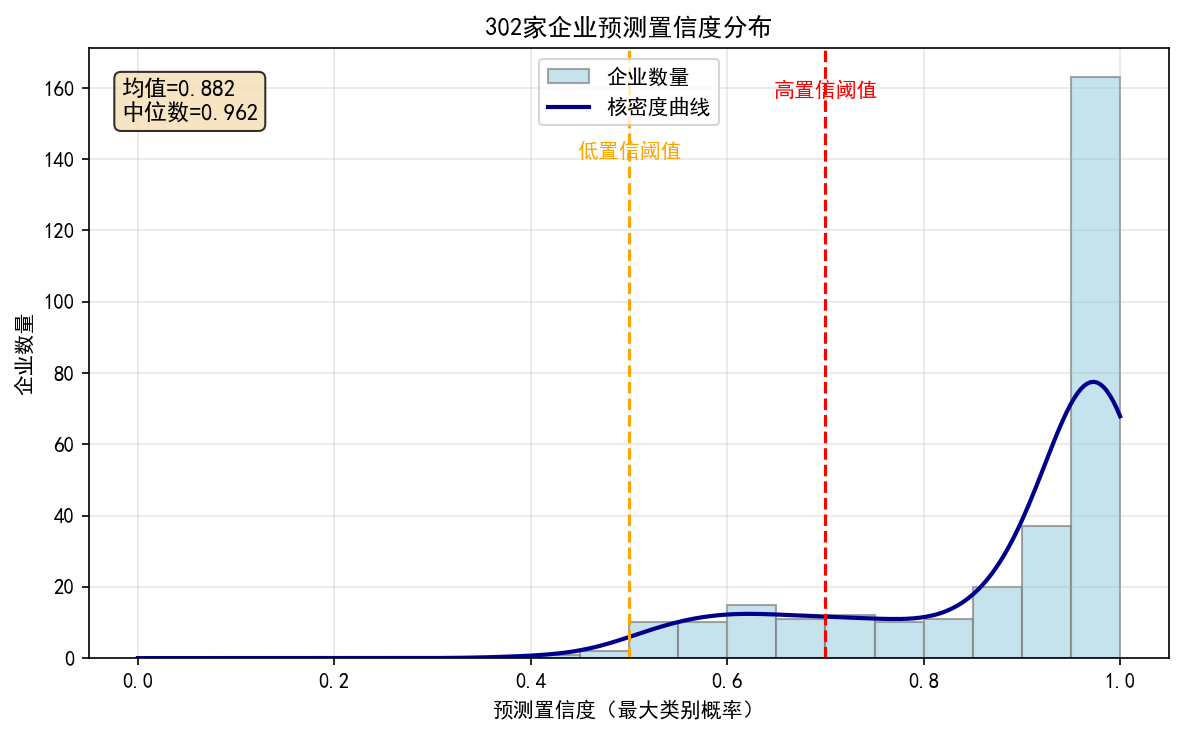
\includegraphics[width=0.7\textwidth]{fig15_confidence_dist.png}
\caption{302家企业预测置信度分布}
\label{fig:confidence}
\end{figure}

\subsubsection{结果分析与验证}

\textbf{标签重构合理性：}新标签$Y'$分布均衡即9/25/50/39，避免了TOPSIS一维投影的极端偏斜。ARI仅0.039揭示客观标准与银行主观判断之间的结构性分歧，印证了问题一B/C中间等级存在严重错配的结论。

\textbf{分类预测可靠性：}91\%的准确率远高于问题一的54.5\%，正确表述为：客观重构标签的内部一致性强，说明熵权聚类标准具有清晰的特征→等级映射关系，分类器能够有效泛化这一映射。302家画像与123家聚类中心高度一致，预测置信度均值0.882，可靠性高。

\textbf{非线性阈值效应：}熵权法中权重极低的稳定度$F_8/F_9$在分类器中重要性排第2、3位，说明信用风险并非线性累积，而是存在临界阈值效应——在线性赋权下企业间差异不大即权重低，但在空间分割中集中度超过临界值会导致信用显著下降。


\section{模型的评价与推广}

\subsection{模型的优点}

本文深挖发票流水背后的供应链网络拓扑结构，构建了更具区分力的企业信用画像。针对传统降维方法导致的标签极端偏斜问题，提出在多维特征空间直接执行加权聚类，在保留多维流形结构的同时实现了标签的均衡分布。研究揭示了信用风险并非线性累积而是存在临界阈值效应，为银行差异化风控提供了理论支撑。

\subsection{模型的缺点}

当前特征体系完全依赖历史交易票据数据，缺乏宏观经济指标与行业属性等外部数据的融合，可能在面对系统性经济波动时表现出滞后性。模型对极少量异常交易行为的鲁棒性仍有待进一步提升。

\subsection{模型的推广}

该模型框架可推广至供应链金融风控与税务信用评价体系中。通过接入更多维度的外部数据源，并结合深度学习技术捕捉更复杂的时序演化规律，能够构建动态化的企业信用监测平台。


\begin{thebibliography}{99}
\addcontentsline{toc}{section}{参考文献}

\bibitem{ref2} 李超杰. 基于机器学习的小微企业信贷供给智能决策系统研究——以"银税互动"政策的共享纳税数据为例[J]. 河海大学学报(哲学社会科学版), 2022, 24(4): 66-74.

\bibitem{ref1} 赵星然, 等. 基于小微企业发票数据的信用风险评价模型研究[J]. 统计与决策, 2022, 38(12).

\bibitem{ref3} Breiman L. Random Forests[J]. Machine Learning, 2001, 45(1): 5-32.

\bibitem{ref4} DeepSeek. DeepSeek V4 Pro 大语言模型[EB/OL]. 2026. 
\bibitem{ref5} 阿里巴巴云计算. 通义千问(Qwen)3.7 Max 大语言模型[EB/OL]. 2026.
\end{thebibliography}


\newpage
\appendix
\renewcommand{\thesection}{附录 \Alph{section}}
\renewcommand{\thesubsection}{\Alph{section}.\arabic{subsection}}
\renewcommand{\thesubsubsection}{\Alph{section}.\arabic{subsection}.\arabic{subsubsection}}
\titleformat{\section}
  {\centering\heiti\zihao{-3}}
  {\thesection}{1em}{}

\section{支撑文件列表}

\begin{table}[H]
\centering
\zihao{5}
\begin{tabular}{lll}
\toprule
文件名 &  说明 \\
\midrule
problem1\_preprocess.py   & 问题一数据清洗与特征提取代码 \\
problem1\_logit.py   & 问题一多元逻辑回归求解代码 \\
problem1\_xgboost.py   & 问题一XGBoost辅助验证代码 \\
problem2\_preprocess.py   & 问题二数据预处理代码 \\
problem2\_entropy\_cluster.py   & 问题二熵权法与加权聚类代码 \\
problem2\_classifier.py   & 问题二有监督分类与预测代码 \\
problem2\_random\_forest.py   & 问题二随机森林对比代码 \\
\bottomrule
\end{tabular}
\end{table}


\section{相关代码}

\lstinputlisting[language=Python, caption={问题一数据清洗与特征提取代码}, firstline=1, lastline=248]{code/problem1_preprocess.py}
\newpage
\lstinputlisting[language=Python, caption={问题一多元逻辑回归求解代码}, firstline=1, lastline=214]{code/problem1_logit.py}

\lstinputlisting[language=Python, caption={问题一XGBoost辅助验证代码}, firstline=1, lastline=87]{code/problem1_xgboost.py}

\lstinputlisting[language=Python, caption={问题二熵权法与加权聚类代码}, firstline=1, lastline=146]{code/problem2_entropy_cluster.py}

\lstinputlisting[language=Python, caption={问题二有监督分类与预测代码}, firstline=1, lastline=157]{code/problem2_classifier.py}

\lstinputlisting[language=Python, caption={问题二随机森林对比代码}, firstline=1, lastline=198]{code/problem2_random_forest.py}

\end{document}